\section{Preliminaries}
\label{sec:preliminaries}

This section fixes the notation, relates the linear and cyclic views, and
states how to interpret a Stainless-verified contract.

\begin{itemize}
  \item Section~2.1 defines one stage and its acceptance predicate.
  \item Section~2.2 defines the finite period and gap cycle.
  \item Section~2.3 maps the proof architecture.
  \item Section~2.4 explains the verification boundary.
\end{itemize}

\subsection{Stage Definition}
\label{sec:stage-definition}

Let a stage $S$ be determined by a current head prime $h$ and the
complete list $\overline{P}$ of primes smaller than $h$. The list is
stored in descending order, but its order does not affect divisibility.
Define

\begin{equation*}
\begin{aligned}
M &= \prod_{q \in \overline{P}} q,
  &&\text{[Tail primorial]} \\
A_S(v) &\Longleftrightarrow
  v \ge h \land
  \forall q \in \overline{P},\ v \not\equiv 0 \pmod q.
  &&\text{[Acceptance]}
\end{aligned}
\end{equation*}

The linear sequence $L=(\ell_k)_{k\ge 0}$ starts at $h$ and repeatedly
selects the least later accepted value:

\begin{equation*}
\begin{aligned}
\ell_0 &= h, \\
\ell_{k+1}
  &= \min\{v\gt\ell_k : A_S(v)\}.
\end{aligned}
\end{equation*}

A stage does \textbf{not} claim that every $\ell_k$ is prime. For
example, the stage with $h=5$ and filters $3,2$ emits
$5,7,11,13,17,19,23,25,\ldots$. The value $25$ survives because the
current head $5$ has not yet been added to the filter list. Prime
generation comes from the chain of stage heads, not from treating all
values in one stage as prime.

The figure below makes this concrete for six early stages: each panel is
a survivor's own leading $100$ values reshaped into a $10\times10$ grid,
colored green where the survivor is actually prime and red where the
current filter set accepted it anyway even though it is composite (stage
$0$, with no filter installed yet, marks every composite integer this
way). Every red cell is exactly the phenomenon named above --- a value
$A_S$ currently accepts that a later stage head will remove.

\begin{figure}[htbp]
\centering
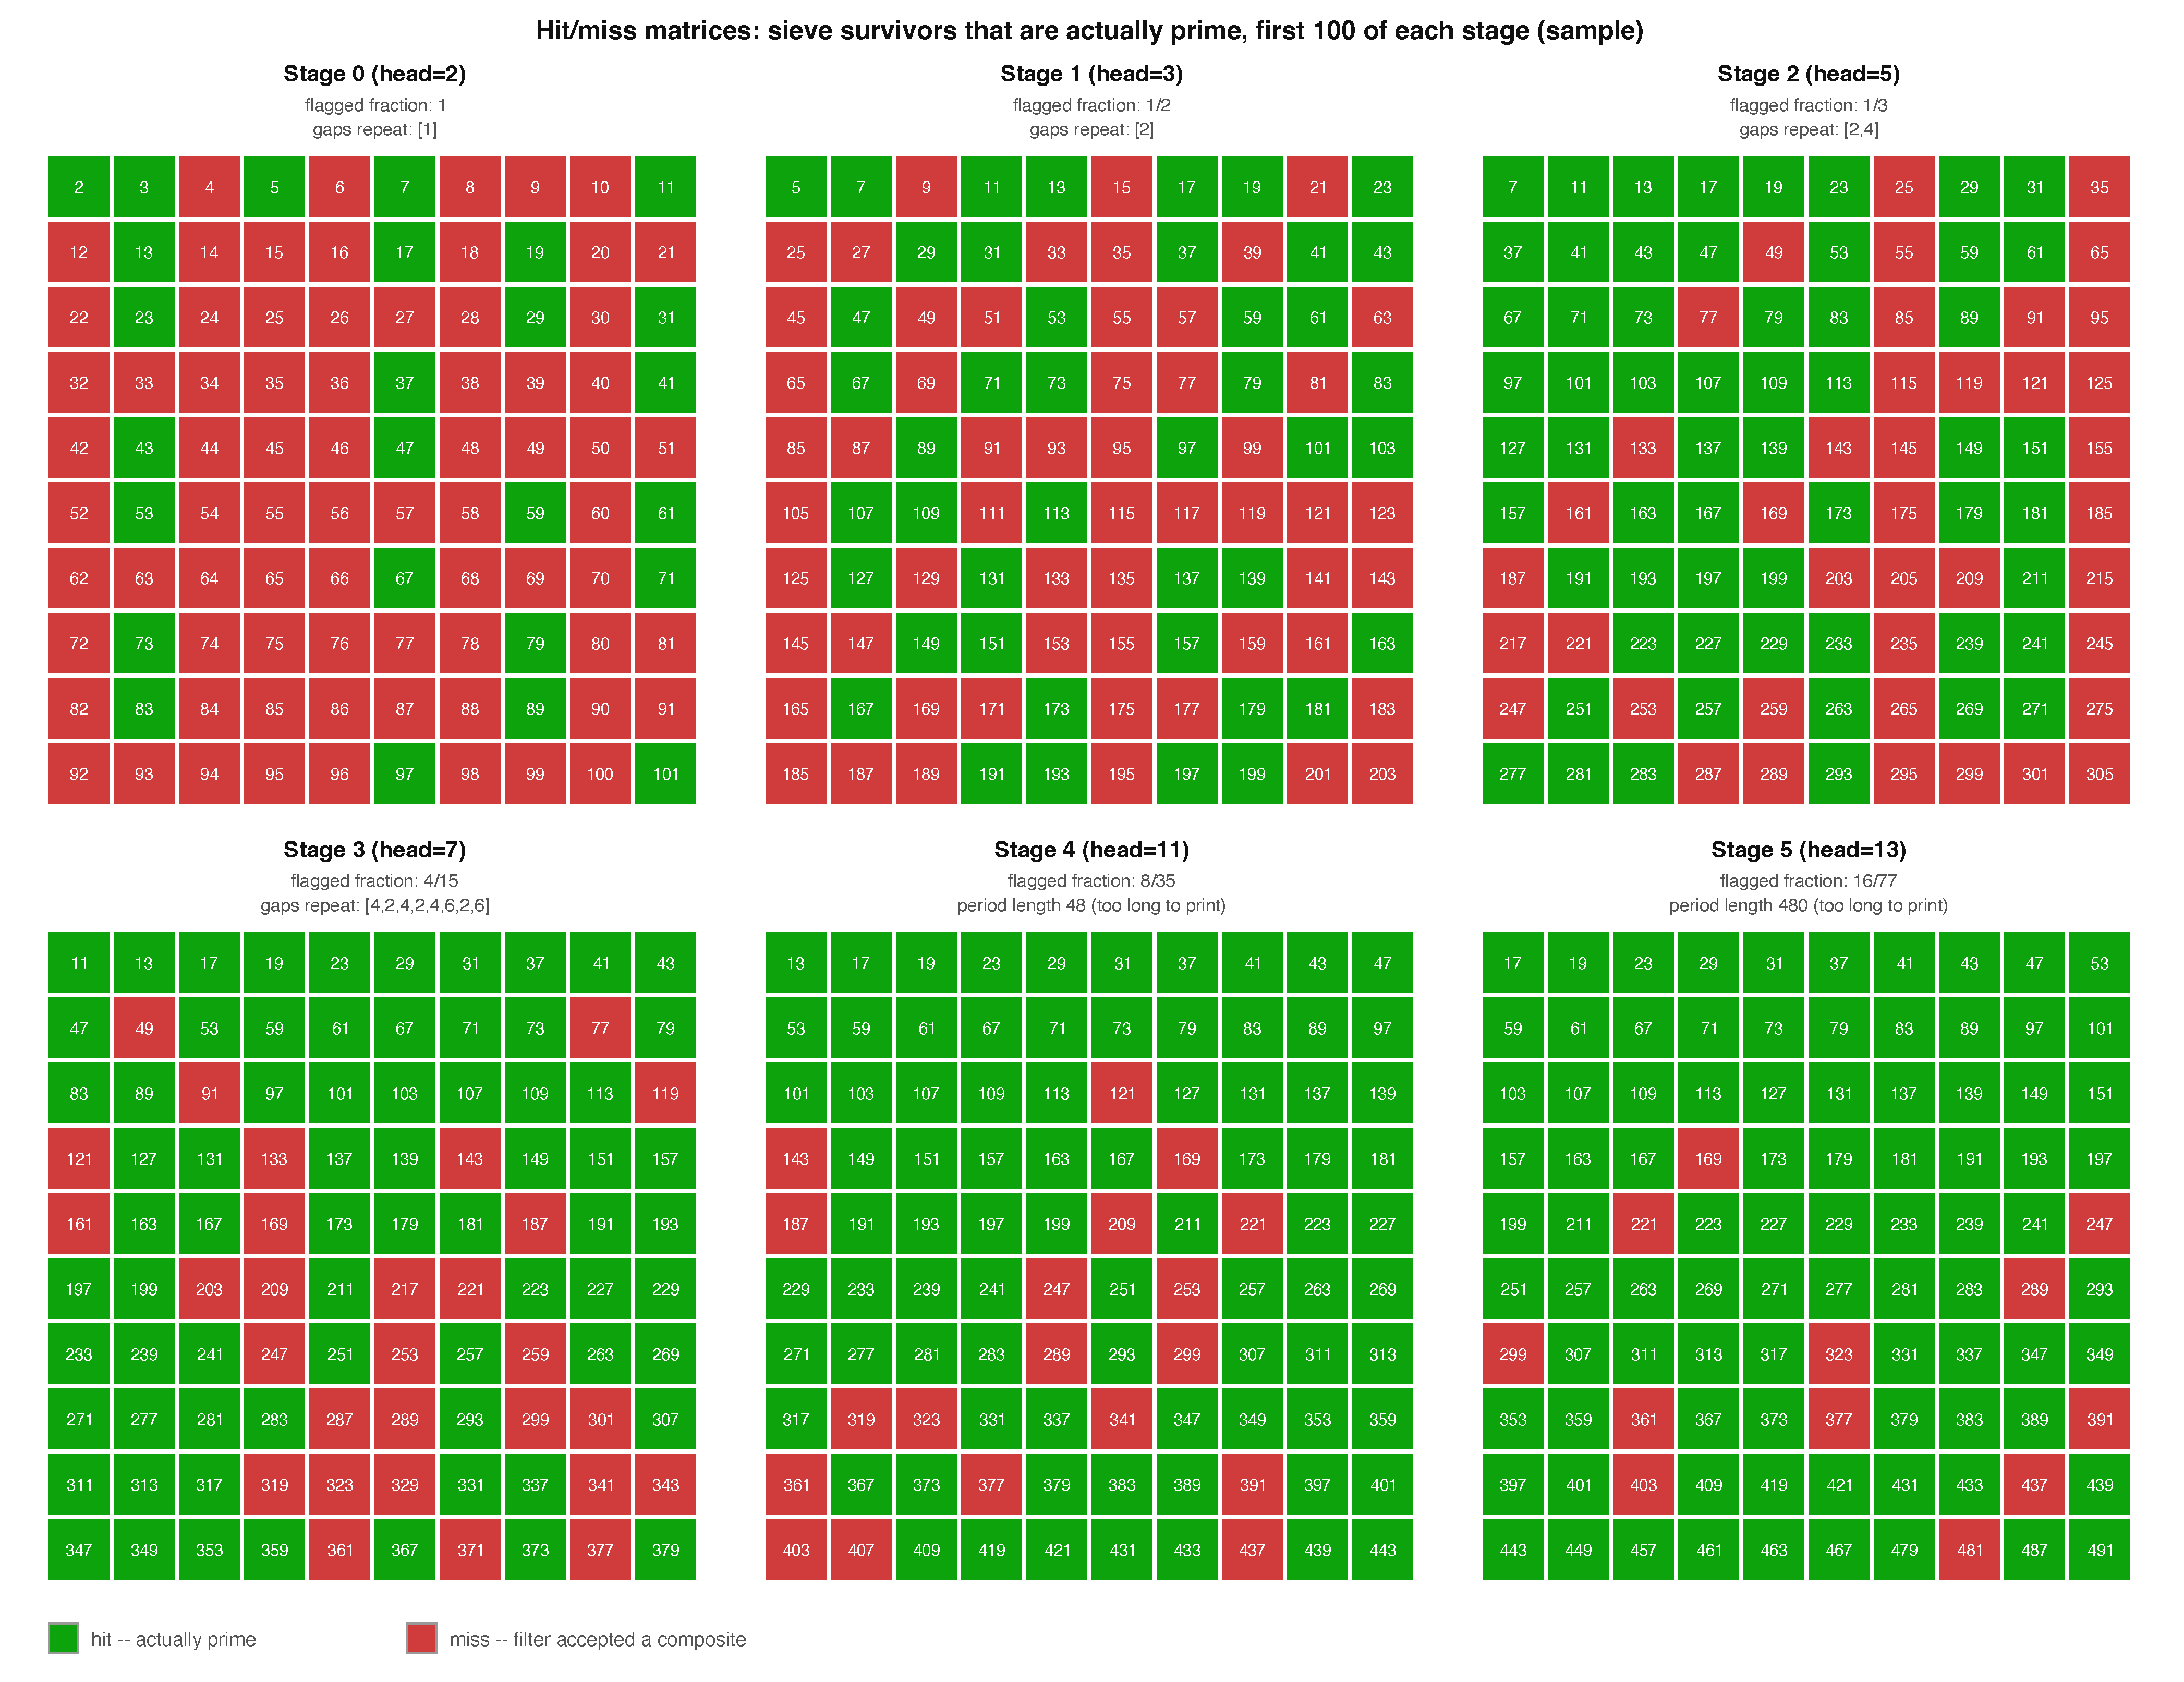
\includegraphics[width=\textwidth]{figures/hit-miss-matrices.pdf}
\caption{Six small hit/miss matrices, one per early stage: green cells
are survivors that are actually prime, red cells are survivors the
current filter set accepted anyway even though they are composite.}
\label{fig:hit-miss-matrices}
\end{figure}

\subsection{Period and Gap Cycle}
\label{sec:period-and-gap-cycle}

Because every $q\in\overline{P}$ divides $M$, acceptance is unchanged by
adding $M$ within the stage domain $v\ge h$:

\begin{equation*}
\begin{aligned}
A_S(v+M)
&\Longleftrightarrow
(v+M)\ge h\ \land\
\forall q\in\overline{P},\ (v+M)\not\equiv0\pmod q \\
&\Longleftrightarrow
v\ge h\ \land\
\forall q\in\overline{P},\ v\not\equiv0\pmod q \\
&\Longleftrightarrow A_S(v).
\end{aligned}
\end{equation*}

Let $T\gt0$ be the unique index satisfying $\ell_T=h+M$. Define one
complete gap list

\begin{equation*}
\begin{aligned}
G &= (g_0,\ldots,g_{T-1}), \\
g_i &= \ell_{i+1}-\ell_i.
\end{aligned}
\end{equation*}

Every gap is positive and the gaps telescope across the period:

\begin{equation*}
\begin{aligned}
g_i &\gt 0, \\
\sum_{i=0}^{T-1} g_i
  &= \ell_T-\ell_0 \\
  &= (h+M)-h \\
  &= M.
\end{aligned}
\end{equation*}

The cycle integral repeatedly adds the entries of $G$. With the indexing
used by the Scala implementation, its position $k-1$ reconstructs
$\ell_k$ for every $k\gt0$.

\subsection{Source Evidence Map}
\label{sec:source-evidence-map}

The proofs below use \texttt{SpecSieveSequence} as the linear
mathematical model of a stage. Separate property objects verify the
period, gap-cycle reconstruction, survivor count, copy-or-merge
transition, next-stage agreement, and head primality facts. The model
does not depend on those property objects; they are source-backed
evidence for the mathematical properties stated in the article.

The construction builds on the verified modulo \cite{mata2026modulo},
list \cite{mata2026lists}, cycle \cite{mata2026cycle}, and cycle-integral
\cite{mata2026integralcycle} foundations.

\subsection{Verification Evidence}
\label{sec:verification-evidence}

Each verified property cited below is tied to a concrete Scala contract
in the repository. The preconditions in those contracts are part of the
theorem statement, and the article states them in mathematical form
before linking to the source. This keeps the mathematical result and the
Stainless evidence aligned without relying on repository-wide
verification-condition totals, which change when unrelated functions are
added. The verification framework's formal foundations are described in
\cite{hamza2019systemfr}.
